% !TEX program = pdflatex
% WordleGym conference poster (A0 portrait, tikzposter).

\documentclass[25pt, a0paper, portrait]{tikzposter}

\usepackage{amsmath, amssymb}
\usepackage{booktabs}
\usepackage{array}
\usepackage{tabularx}
\usepackage{xstring}
\usepackage{tikz}
\usepackage{qrcode}
\usepackage{microtype}
\usepackage{graphicx}

% Modern sans-serif default
\usepackage[scaled=0.95]{helvet}
\renewcommand{\familydefault}{\sfdefault}
\usepackage{sfmath}

\tikzposterlatexaffectionproofoff

% ── Theme ─────────────────────────────────────────────────────────
\definecolor{dukenavy}{HTML}{012169}
\definecolor{dukegold}{HTML}{C29C57}
\definecolor{accentteal}{HTML}{4A8FB5}
\definecolor{neutralgray}{HTML}{4A5568}
\definecolor{paleNavy}{HTML}{E8EDF5}

\usetheme{Simple}
\usebackgroundstyle{Empty}
\usetitlestyle{Filled}

% Clean block style: filled navy title bar, no body border, no dividers.
% titleinnersep keeps the navy bar visually proportionate to the body text;
% the explicit \Large in blocktitlestyle stops tikzposter from letting the
% bar swell with the 25pt base font.
\defineblockstyle{Clean}{
  titlewidthscale=1, bodywidthscale=1, titleleft,
  titleoffsetx=0pt, titleoffsety=0pt,
  bodyoffsetx=0mm, bodyoffsety=0mm,
  bodyverticalshift=0mm, roundedcorners=0,
  linewidth=0pt, titleinnersep=4mm, bodyinnersep=3mm
}{
  \ifBlockHasTitle
    \draw[draw=none, fill=blocktitlebgcolor]
      (blocktitle.south west) rectangle (blocktitle.north east);
  \fi
}
\useblockstyle{Clean}
% tikzposter sizes block titles at \Huge by default, which is too tall for
% A0 once the body text is set at the document's 25pt base. Wrap titles via
% this helper so every navy bar is proportionate to its body.
\newcommand{\btitle}[1]{\large\bfseries #1}

% Inner block: filled teal title bar (one hierarchy step lighter than navy).
\defineinnerblockstyle{Sub}{
  titlewidthscale=1, bodywidthscale=1, titlecenter,
  titleoffsetx=0pt, titleoffsety=0pt,
  bodyoffsetx=0mm, bodyoffsety=0mm,
  bodyverticalshift=0mm, roundedcorners=0,
  linewidth=0pt, titleinnersep=3mm, bodyinnersep=4mm
}{
  \ifInnerBlockHasTitle
    \draw[draw=none, fill=innerblocktitlebgcolor]
      (innerblocktitle.south west) rectangle (innerblocktitle.north east);
  \fi
}
\useinnerblockstyle{Sub}

% Inline subsection bar: slim teal banner, full width.
\newcommand{\subbar}[1]{%
  \par\noindent
  \setlength{\fboxsep}{2.5mm}%
  \colorbox{accentteal}{%
    \parbox{\dimexpr\linewidth-2\fboxsep\relax}{%
      \centering\color{white}\bfseries #1}}%
  \setlength{\fboxsep}{3pt}%
  \par
}

\colorlet{titlefgcolor}{white}
\colorlet{titlebgcolor}{dukenavy}
\colorlet{backgroundcolor}{white}
\colorlet{framecolor}{white}
\colorlet{blocktitlefgcolor}{white}
\colorlet{blocktitlebgcolor}{dukenavy}
\colorlet{blockbodyfgcolor}{black!85}
\colorlet{blockbodybgcolor}{white}
\colorlet{innerblocktitlebgcolor}{accentteal}
\colorlet{innerblocktitlefgcolor}{white}
\colorlet{innerblockbodybgcolor}{white}
\colorlet{notefgcolor}{white}
\colorlet{notebgcolor}{dukenavy!85}

% ── Strategy colour palette (mirrors the web and supplementary writeup) ───────
\definecolor{stratEntropy}{HTML}{2563EB}
\definecolor{stratPosteriorExp}{HTML}{0891B2}
\definecolor{stratMinimax}{HTML}{EF4444}
\definecolor{stratLetterFreq}{HTML}{F59E0B}
\definecolor{stratRandom}{HTML}{94A3B8}
\definecolor{stratEvilDP}{HTML}{16A34A}

% ── Wordle tile graphics ──────────────────────────────────────────
\definecolor{wordleGreen}{HTML}{6AAA64}
\definecolor{wordleYellow}{HTML}{C9B458}
\definecolor{wordleGray}{HTML}{787C7E}
\definecolor{wordleEmpty}{HTML}{D3D6DA}

\newlength{\wtilesize}\setlength{\wtilesize}{14mm}
\newcommand{\wtilefont}{\bfseries\sffamily}

\newcommand{\wtileC}[3]{%
  \tikz[baseline=(t.base)]{
    \node[fill=#2, text=#3, font=\wtilefont,
          minimum width=\wtilesize, minimum height=\wtilesize,
          inner sep=0pt, outer sep=0.6pt] (t) {\MakeUppercase{#1}};%
  }%
}
\newcommand{\wG}[1]{\wtileC{#1}{wordleGreen}{white}}
\newcommand{\wY}[1]{\wtileC{#1}{wordleYellow}{white}}
\newcommand{\wB}[1]{\wtileC{#1}{wordleGray}{white}}
\newcommand{\wE}[1]{\wtileC{#1}{wordleEmpty}{black!55}}

\newcommand{\wrow}[2]{%
  \StrChar{#1}{1}[\wxA]\StrChar{#2}{1}[\wyA]%
  \StrChar{#1}{2}[\wxB]\StrChar{#2}{2}[\wyB]%
  \StrChar{#1}{3}[\wxC]\StrChar{#2}{3}[\wyC]%
  \StrChar{#1}{4}[\wxD]\StrChar{#2}{4}[\wyD]%
  \StrChar{#1}{5}[\wxE]\StrChar{#2}{5}[\wyE]%
  \mbox{%
    \csname w\wyA\endcsname{\wxA}%
    \csname w\wyB\endcsname{\wxB}%
    \csname w\wyC\endcsname{\wxC}%
    \csname w\wyD\endcsname{\wxD}%
    \csname w\wyE\endcsname{\wxE}%
  }%
}

% ── Compact tile rows for the inline strategy traces ──────────────
\newlength{\wsmallsize}\setlength{\wsmallsize}{7mm}
\newcommand{\wtileS}[3]{%
  \tikz[baseline=(t.base)]{
    \node[fill=#2, text=#3, font=\wtilefont\footnotesize,
          minimum width=\wsmallsize, minimum height=\wsmallsize,
          inner sep=0pt, outer sep=0.3pt] (t) {\MakeUppercase{#1}};%
  }%
}
\newcommand{\wsG}[1]{\wtileS{#1}{wordleGreen}{white}}
\newcommand{\wsY}[1]{\wtileS{#1}{wordleYellow}{white}}
\newcommand{\wsB}[1]{\wtileS{#1}{wordleGray}{white}}
\newcommand{\wsrow}[2]{%
  \StrChar{#1}{1}[\sxA]\StrChar{#2}{1}[\syA]%
  \StrChar{#1}{2}[\sxB]\StrChar{#2}{2}[\syB]%
  \StrChar{#1}{3}[\sxC]\StrChar{#2}{3}[\syC]%
  \StrChar{#1}{4}[\sxD]\StrChar{#2}{4}[\syD]%
  \StrChar{#1}{5}[\sxE]\StrChar{#2}{5}[\syE]%
  \mbox{%
    \csname ws\syA\endcsname{\sxA}%
    \csname ws\syB\endcsname{\sxB}%
    \csname ws\syC\endcsname{\sxC}%
    \csname ws\syD\endcsname{\sxD}%
    \csname ws\syE\endcsname{\sxE}%
  }%
}

% Larger tiles for the poster title.
\newlength{\wtitlesize}\setlength{\wtitlesize}{22mm}
\newcommand{\wtitleTile}[3]{%
  \tikz[baseline=(t.base)]{
    \node[fill=#2, text=#3, font=\bfseries\sffamily\fontsize{47}{51}\selectfont,
          minimum width=\wtitlesize, minimum height=\wtitlesize,
          inner sep=0pt, outer sep=1.3pt] (t) {#1};%
  }%
}
\newcommand{\titleWordle}{%
  \mbox{%
    \wtitleTile{W}{wordleGreen}{white}%
    \wtitleTile{O}{wordleYellow}{white}%
    \wtitleTile{R}{wordleGray}{white}%
    \wtitleTile{D}{wordleGreen}{white}%
    \wtitleTile{L}{wordleYellow}{white}%
    \wtitleTile{E}{wordleGreen}{white}%
  }%
}

% ── Title block ───────────────────────────────────────────────────
% Override tikzposter's default small-caps title rendering with our own.
\settitle{%
  \color{titlefgcolor}%
  \centering
  {\titleWordle\hspace{5mm}{\fontsize{64}{74}\selectfont\bfseries Gym: Benchmarking Wordle Strategies}}\par\vspace{2mm}
  {\fontsize{40}{48}\selectfont under Standard, Adversarial, and Hidden-Mode Play}\par\vspace{8mm}
  {\Large\bfseries Michael Wang} \quad\textbullet\quad
  {\large Math 242, Duke University, Spring 2026} \quad\textbullet\quad
  {\large\ttfamily michael.wang@duke.edu}\par\vspace{2mm}
  {\large \ttfamily github.com/Michael-OvO/WordleGym \quad{\normalfont\textbullet}\quad wordlegym.vercel.app}\par
}

\begin{document}

\maketitle[width=0.97\textwidth, titletotopverticalspace=4mm,
           titletoblockverticalspace=6mm]

%====================================================================
\begin{columns}
\column{0.42}

\block{\btitle{The Problem}}{
Classic Wordle gives six guesses; here we report solve depth so weak baselines can run past six instead of tying as failures. The answer is one of $2{,}315$ five-letter English words. After each guess, tiles paint back: \textcolor{wordleGreen}{\textbf{green}} if right, \textcolor{wordleYellow}{\textbf{yellow}} if misplaced, and \textcolor{wordleGray}{\textbf{gray}} if absent. \mbox{\textbf{WordleGym}} benchmarks ten strategies, summarized by six representative policies across three game flavors.
\smallskip

\textbf{Standard.} The answer is fixed before you start. Feedback is honest. The game most humans play.
\smallskip

\textbf{Evil.} The host cheats. After every guess, they pick the feedback that keeps the most candidate answers alive. ``The answer'' is whatever's most adversarial given history. In worst-case solve depth, this turns out to be easier than honest Standard Wordle.
\smallskip

\textbf{Unknown.} A coin flip at game-start picks Standard or Evil; you don't know which. Each turn's feedback is more likely under one mode than the other, so Bayes does the work --- but does the right policy hedge?
}

\block{\btitle{Six Strategy Families}}{
Every strategy answers the same question --- ``which legal guess do I play next?'' --- with a different scoring rule. Let $A$ be the answer list, $G$ the legal guess list, $C\subseteq A$ the candidates still consistent with feedback, and $B_r(C,g)$ the subset that would produce pattern $r$ against guess $g\in G$; $p(r)=|B_r|/|C|$.
\smallskip

\renewcommand{\arraystretch}{1.28}
\newcolumntype{S}{>{\ttfamily\raggedright\arraybackslash}p{0.34\linewidth}}
\newcolumntype{F}{>{\raggedright\arraybackslash}p{0.57\linewidth}}
\begin{tabular}{@{} S F @{}}
\toprule
\normalfont\bfseries Strategy & \bfseries Score used to choose the next guess\\
\midrule
random-valid & uniform pick from $C$\\
letter-frequency & $\arg\max_g\,\mathrm{freq}(g;C)$\\
expected-entropy & $\arg\max_g \sum_r p(r)\log_2(1/p(r))$\\
minimax & $\arg\min_g \max_r |B_r|$\\
posterior-expectimax & $\arg\min_g\,[qE(g)+(1-q)|T(C,g)|]$, where $E(g)=\sum_r |B_r|^2/|C|$\\
evil-dp & beam-memoised DP for $D(C)$ \quad(Evil only)\\
\bottomrule
\end{tabular}
\smallskip

\texttt{expected-entropy} balances buckets; \texttt{minimax} guards the largest one. \texttt{posterior-expectimax} hedges by $q$; \texttt{evil-dp} is the only DP-style policy reported here.
}

\column{0.58}

\block{\btitle{Three Recurrences}}{
Read each recurrence as the same recipe: choose the legal guess with the smallest future cost, pay $1$ turn now, and recurse only if the feedback is not all-green $\gamma$. With one candidate left, $V(\{w\})=D(\{w\})=1$.

\subbar{Standard \,---\, honest feedback: average over possible buckets}
\vspace{-2mm}
\[
  V(C) = \min_{g}\!\Bigl[\,1 + \!\!\sum_{r \ne \gamma,\,B_r \ne \emptyset}\! \tfrac{|B_r|}{|C|}\,V(B_r)\Bigr]
\]

\subbar{Evil \,---\, adversary: continue in the largest remaining bucket}
\vspace{-2mm}
\[
  D(C)=\min_g\bigl[\,1+D(T(C,g))\bigr],
  \qquad
  T(C,g)=\text{largest }B_r\text{, tied by fewer greens/yellows.}
\]

\subbar{Unknown \,---\, hidden mode: average using the current posterior $q$}
\vspace{-2mm}
\[
  V_U(C,q)=\min_g\Bigl[1+\!\!\sum_{r\ne\gamma}P(r\mid C,q,g)\,V_U(C_r,q_r)\Bigr]
\]

Here $C_r$ is the candidate state after feedback $r$, and $q_r$ is the Bayes-updated belief that the game is Standard. Evil follows one forced branch; Standard and Unknown average over branches. That is why $D$ fits on a laptop: Evil reaches only ${\sim}2{,}948$ subsets, while Standard expands over weighted partitions. We use the published $V(A){=}3.421$ as the comparison target.
}

\block{\btitle{Benchmark Results}}{
\renewcommand{\arraystretch}{1.18}
\newcolumntype{Y}{>{\centering\arraybackslash}X}
\begin{tabularx}{\linewidth}{@{} l Y Y Y Y Y Y @{}}
\toprule
& \multicolumn{2}{c}{Standard} & \multicolumn{2}{c}{Evil} & \multicolumn{2}{c}{Unknown}\\
\cmidrule(lr){2-3}\cmidrule(lr){4-5}\cmidrule(lr){6-7}
Strategy & Mean & WC & Depth & WC & Mean & WC\\
\midrule
\texttt{expected-entropy}     & \textbf{3.465} & 6 & 5 & 5 & \textbf{4.232} & 6\\
\texttt{posterior-hybrid}     & \textbf{3.465} & 6 & 5 & 5 & 4.237 & 6\\
\texttt{posterior-expectimax} & 3.485 & \textbf{5} & 5 & 5 & 4.248 & \textbf{5}\\
\texttt{minimax}              & 3.573 & 6 & 5 & 5 & 4.287 & 6\\
\texttt{letter-frequency}     & 3.587 & 8 & 5 & 5 & 4.294 & 8\\
\texttt{random-valid}         & 4.124 & 9 & 7 & 7 & 4.996 & 9\\
\midrule
\texttt{evil-dp} (optimal)    & ---            & ---       & \textbf{4} & \textbf{4} & ---            & ---       \\
Published optimum             & \textbf{3.421} & \textbf{5}& \textbf{4} & \textbf{4} & ---            & ---       \\
\bottomrule
\end{tabularx}

\smallskip
Representative rows from the ten-strategy benchmark: 2{,}315 Standard answers, deterministic Evil, 2{,}316 Unknown games. Evil has one forced path per strategy, so Depth=WC. Bold = best. \texttt{expected-entropy} and \texttt{posterior-hybrid} average 1.3\% above published $V(A){=}3.421$.
}

\end{columns}

%====================================================================
\block{\btitle{Inside the Argmin --- Why the Algorithm Picks SOARE}}{
\centering
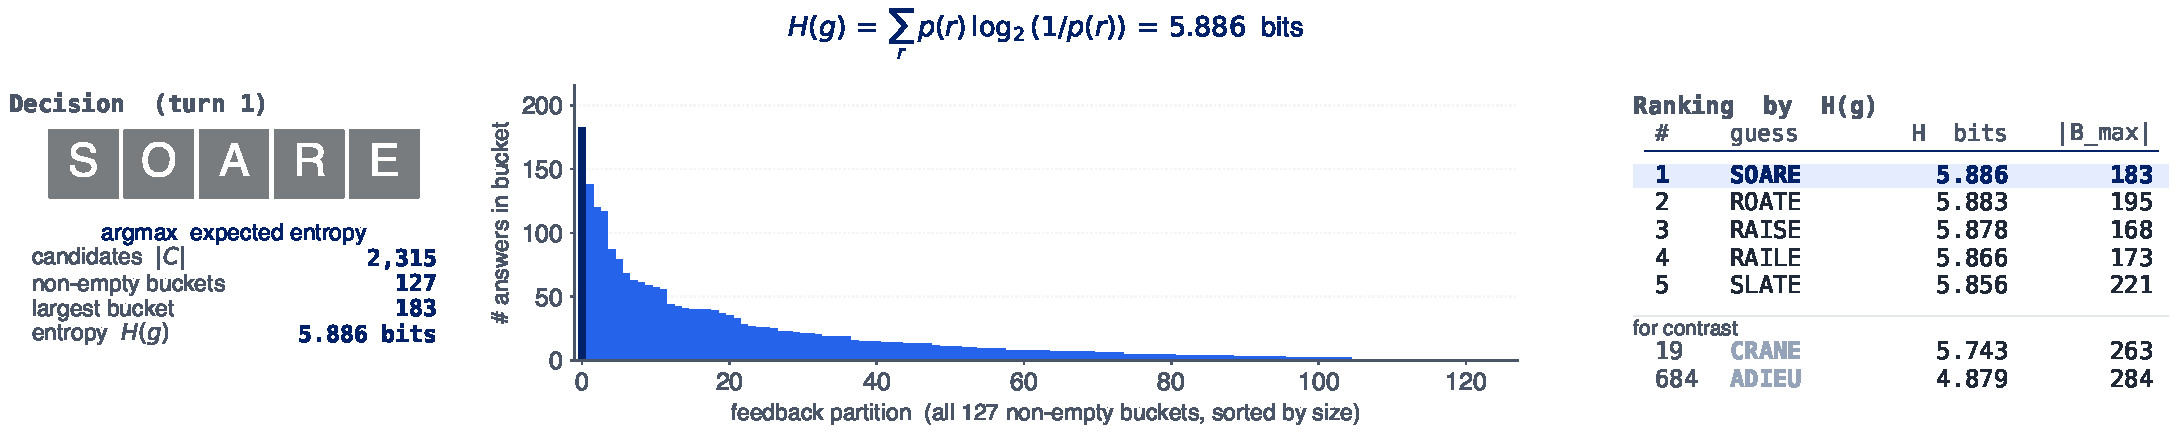
\includegraphics[width=\linewidth]{figures/entropy_mechanism.pdf}\par
\vspace{1mm}
\raggedright
For a fixed guess, group the $2{,}315$ answers by the feedback pattern they'd produce --- the middle panel is \textbf{SOARE}'s histogram. A balanced histogram means whatever feedback comes back, you've eliminated about the same number of candidates --- exactly Shannon's $H(g){=}\sum p(r)\log_2(1/p(r))$, which \texttt{expected-entropy} argmaxes. \textbf{SOARE} wins at $5.886$ bits; \textbf{CRANE} has a giant bucket of $263$ (worst case, barely moved); \textbf{ADIEU}'s vowel-heavy spread collapses into $80$ buckets. The other strategies share the same histogram with different objectives: \texttt{minimax} minimises the tallest bar; \texttt{letter-frequency} counts shared letters; \texttt{evil-dp} recurses over Evil's forced bucket.
}

%====================================================================
\begin{columns}
\column{0.5}

\block{\btitle{Average vs. Worst-Case Trade-Off}}{
\centering
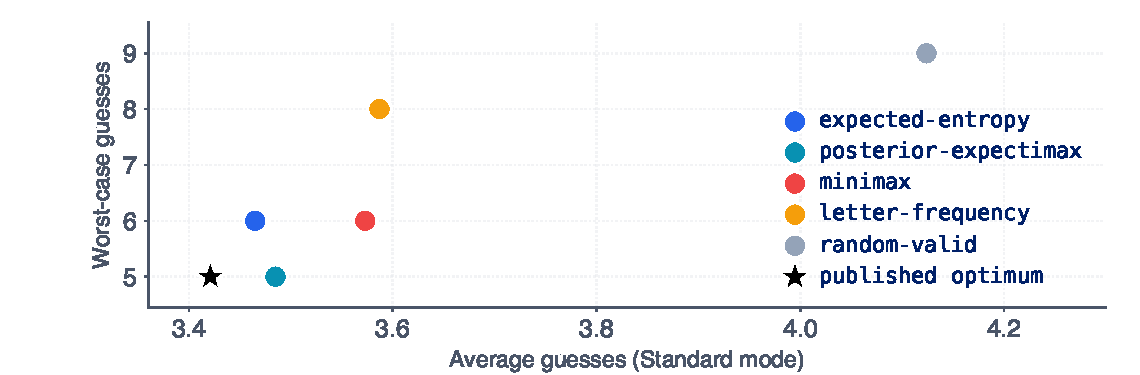
\includegraphics[width=\linewidth]{figures/pareto_scatter.pdf}\par
\vspace{1mm}
\raggedright
Each dot is a strategy at (mean guesses, worst-case guesses) --- lower-left is better, and a point dominates another if it is no worse on both axes. The headline: average and worst-case are different objectives. \texttt{expected-entropy} wins on average; \texttt{posterior-expectimax} shaves one worst-case turn for $0.02$ guesses on average. The star is the published Standard optimum --- the unreachable corner one-ply heuristics chase.
}

\column{0.5}

\block{\btitle{Why Mode-Blending Fails --- the Posterior Collapses}}{
\centering
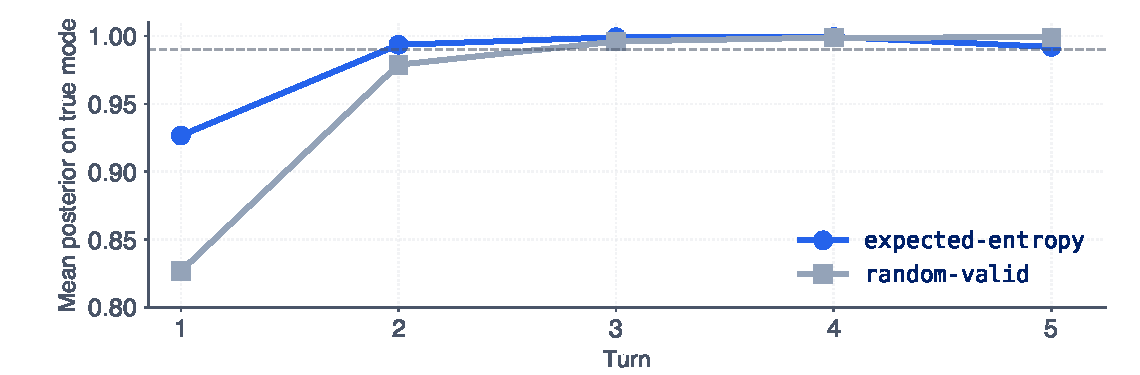
\includegraphics[width=\linewidth]{figures/posterior_concentration.pdf}\par
\vspace{1mm}
\raggedright
In Unknown mode you don't know if it's Standard or Evil; each guess's feedback is more likely under one, and Bayes does the rest. The y-axis is the mean posterior assigned to the \textit{true} mode. \texttt{expected-entropy} crosses $0.99$ between turn~$1$ and~$2$; even \texttt{random-valid} catches up by turn~$3$. Mode-aware one-ply policies hedge only while uncertain --- a window that usually closes by turn~$2$, so \texttt{posterior-expectimax}'s blend has little room to help.
}

\end{columns}

%====================================================================
\begin{columns}
\column{0.70}

\block{\btitle{Findings}}{
{\small
\textbf{1.~One-ply lookahead is plenty.} In the table, \texttt{expected-entropy} averages $3.465$ guesses vs.\ published optimum $3.421$ --- within $1.3\%$, no recursive Standard DP.\\
\textbf{2.~Average and worst-case differ.} The Pareto figure shows \texttt{posterior-expectimax} pays $+0.02$ mean for one fewer worst-case turn. No free lunch.\\
\textbf{3.~Evil is \textit{easier} than Standard.} $D(A){=}4 < W(A){=}5$: the deterministic largest-bucket adversary cannot force more than four guesses; the worst honest Standard answer needs five.\\
\textbf{4.~Mode-blending is a mirage.} The posterior figure shows mode probability above $99\%$ by turn $2$, so one-ply Unknown policies have little time to exploit hedging.
}
}

\column{0.30}

\block{\btitle{Code, Demo \& References}}{
\centering
\setlength{\tabcolsep}{4pt}
\renewcommand{\arraystretch}{1.0}
\begin{tabular}{@{}c@{\hspace{6mm}}c@{}}
\qrcode[height=1.45cm]{https://github.com/Michael-OvO/WordleGym} &
\qrcode[height=1.45cm]{https://wordlegym.vercel.app/}\\[0.5mm]
{\small\ttfamily github.com/} & {\small\ttfamily wordlegym}\\[-1pt]
{\small\ttfamily Michael-OvO/WordleGym} & {\small\ttfamily .vercel.app}\\
\end{tabular}

\raggedright\footnotesize
\textit{Supplement:} \texttt{wordle\_gym\_writeup.pdf} and \texttt{.tex}.\\
\textit{Refs:} Bertsimas--Paskov 2025, doi:10.1287/opre.2022.0434; Selby 2022; Sanderson 2022; Shannon 1948.
}

\end{columns}

\end{document}
